\section{Simulation}
This section details the Monte Calro simulation used for this analysis.
%The purpose of those MC simulation is as follows:
%\begin{itemize}
%\item Acceptance Correction
%\item Kinematic Fit
%\end{itemize}

\begin{table}[]
  \centering
  \caption{simulation setup}
  \begin{tabular}{l|l} \hline
  GEANT4 version & 4.10.01p1   \\ \hline\hline
  Physics list  &  QGSP\_BERT\_HP   \\ \hline\hline
  Beam Momentum & 1.000 GeV/c (fixed)  \\ \hline\hline 
  \end{tabular}
\end{table}

\subsection{CDS configuration}
The Solenoid magnet modeled in GEANT4 is updated from previous analysis\cite{hashimoto:2013dt,sada:2017dt,yamaga:2018dt}.
From this analysis, the Bobbin layer and the Coil are implemented in Doraemon to evaluate the effect of material to the neutron analysis.
 




%$\Sigma^+\pi^- n$ and $\Sigma^-\pi^+ n$ events are generated with isotropic phase-space distribution.

%\begin{figure}
%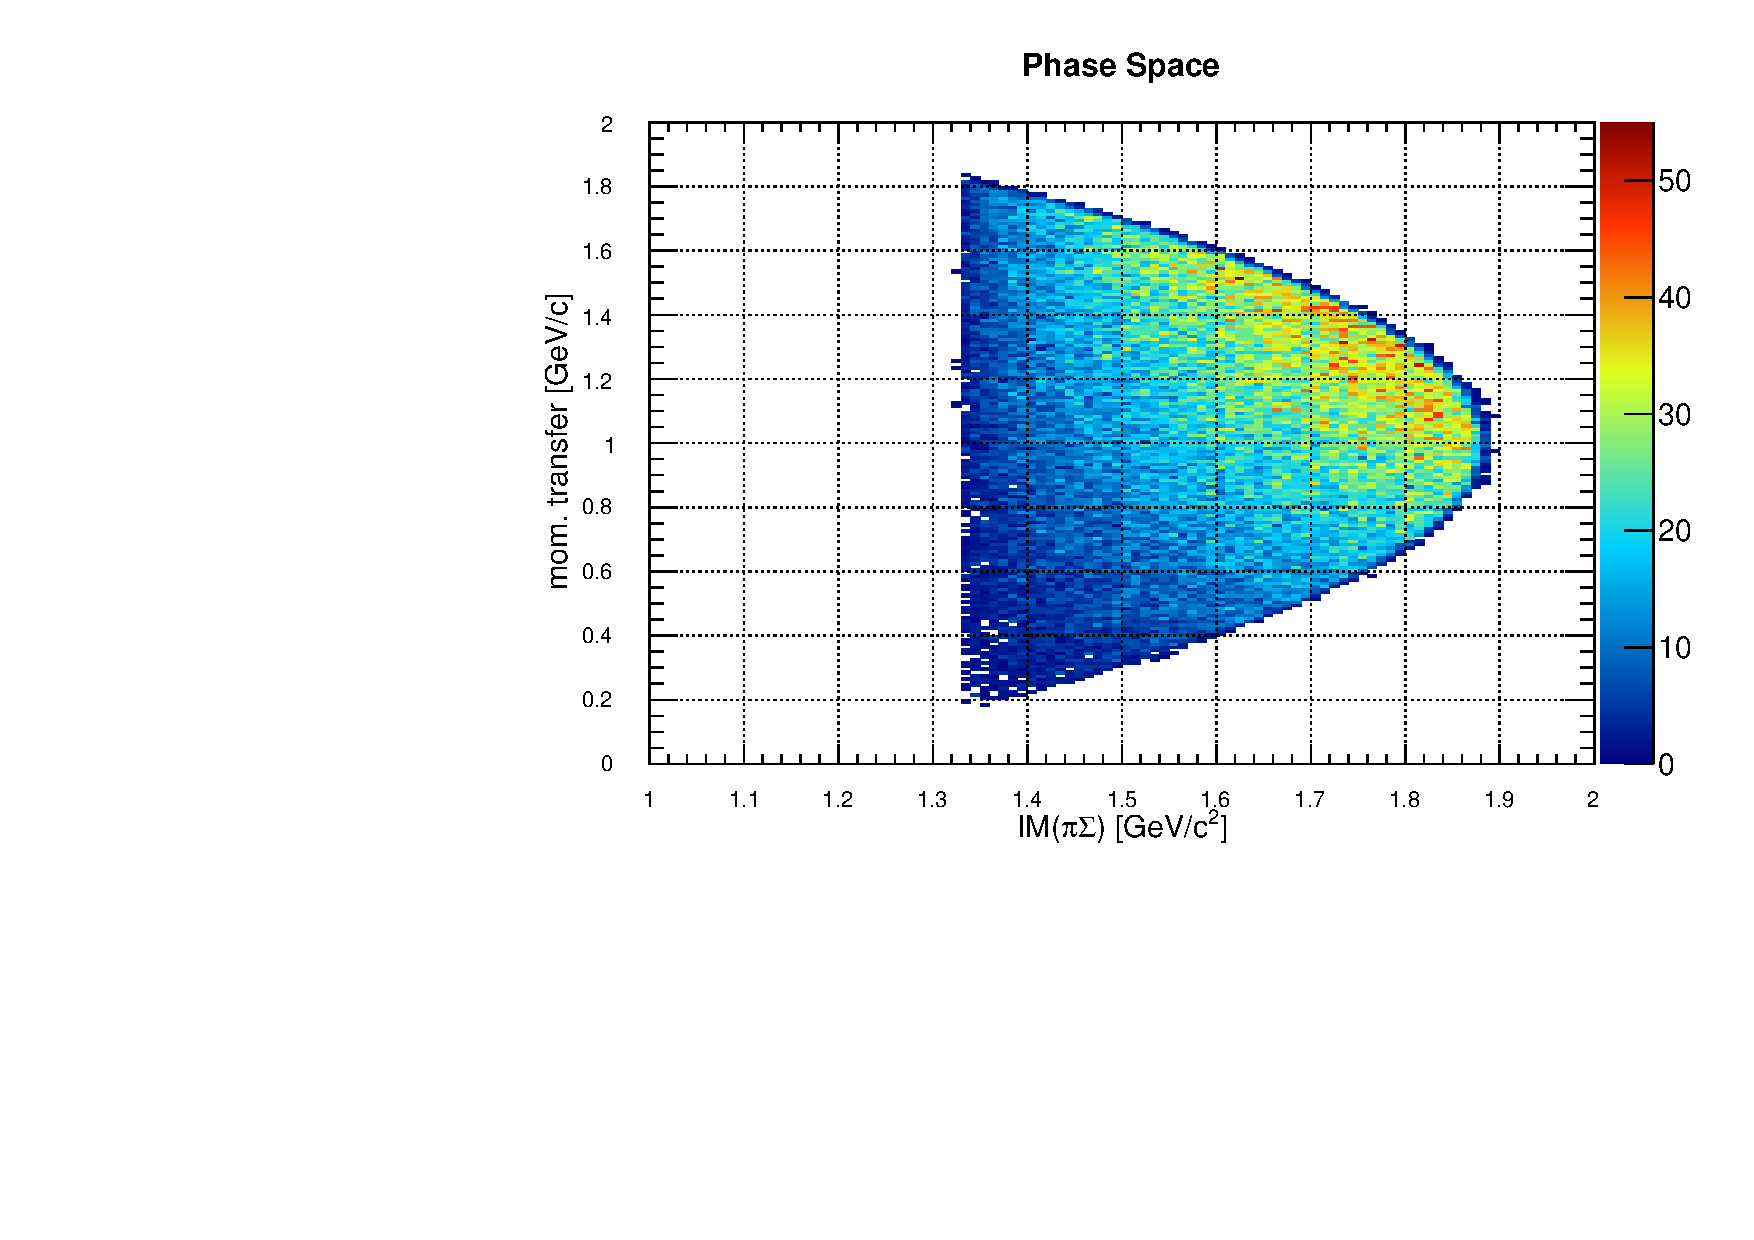
\includegraphics[width=0.45\linewidth]{PSSp.pdf}
%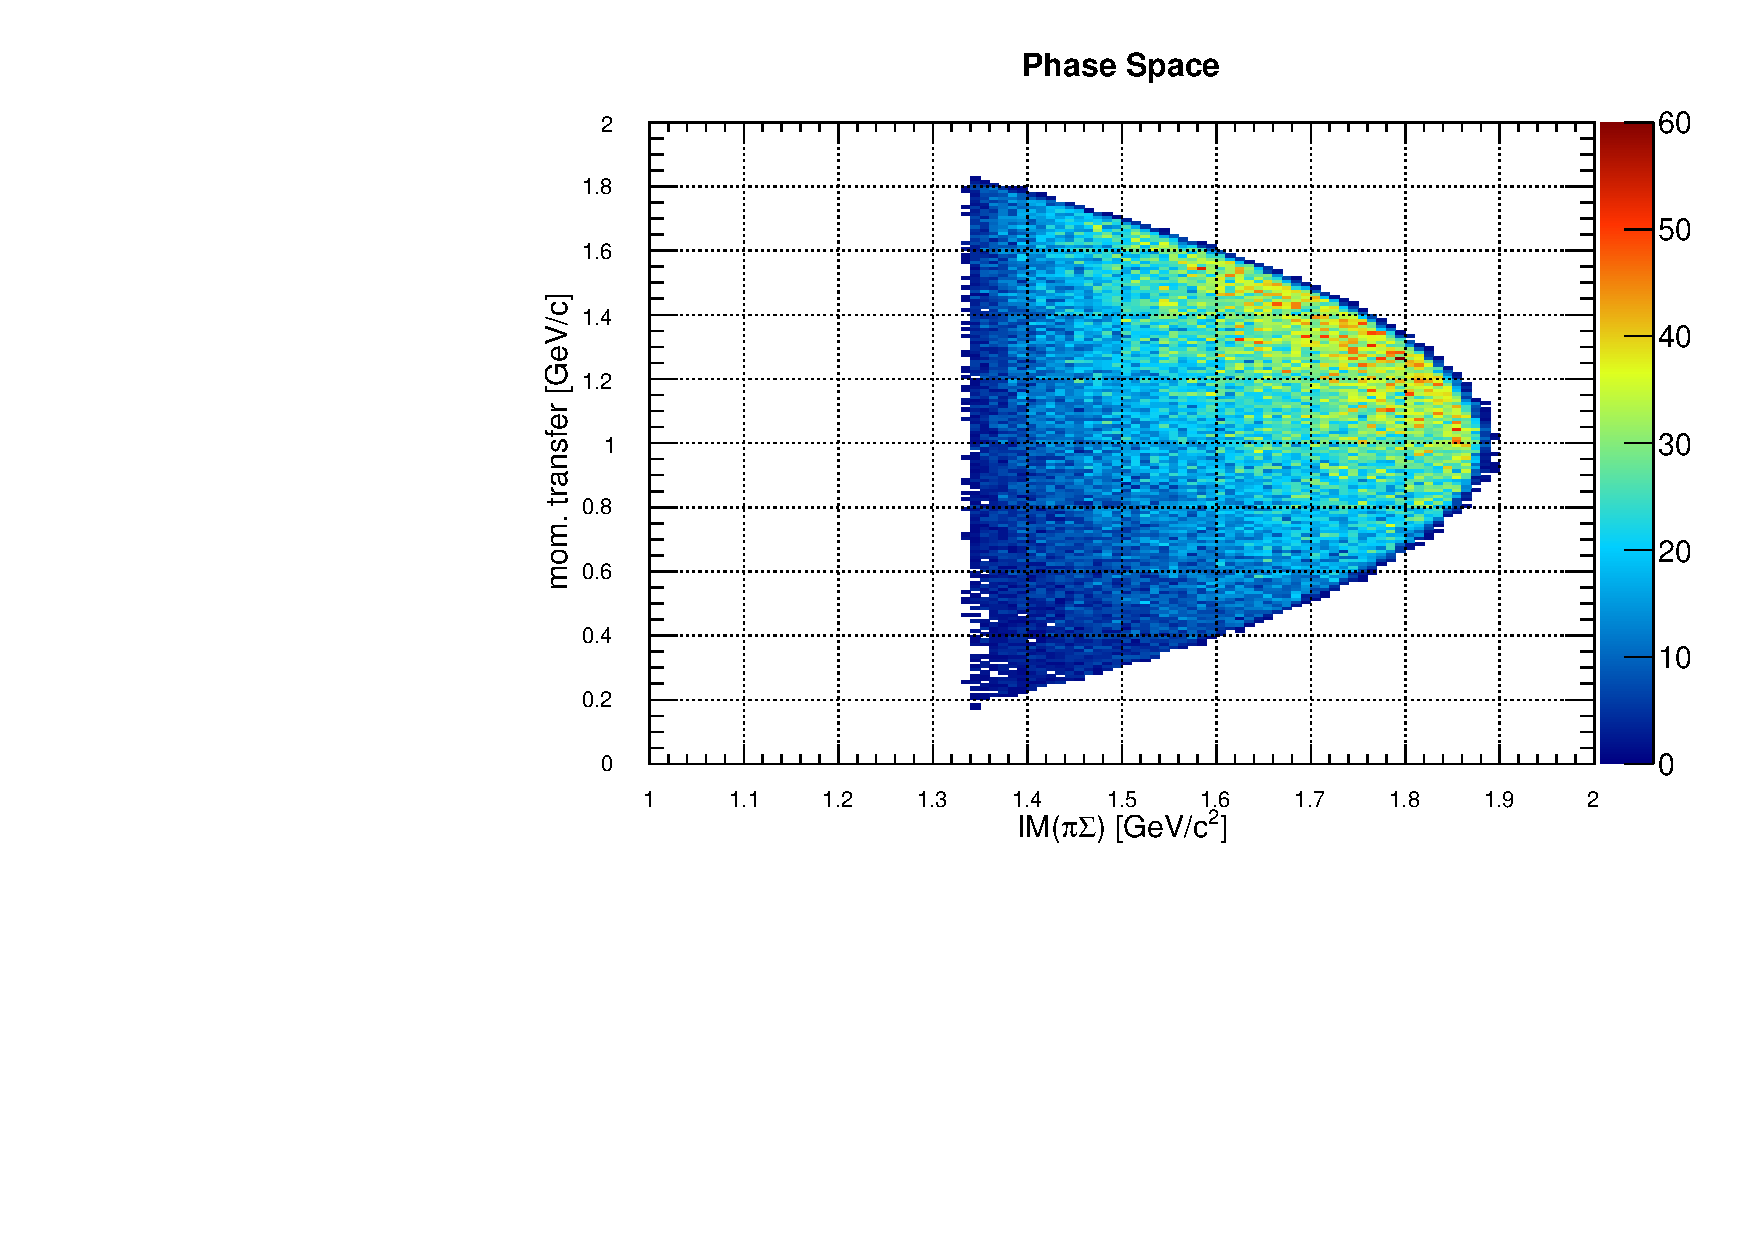
\includegraphics[width=0.45\linewidth]{PSSm.pdf}
%\caption{Phase Space distribution of $\Sigma^+$ mode (left) and $\Sigma^-$ mode (right).}
%\end{figure}




%\subsection{Covariance matrix of the kinematic fit}

